\documentclass[1p]{elsarticle_modified}
%\bibliographystyle{elsarticle-num}

%\usepackage[colorlinks]{hyperref}
%\usepackage{abbrmath_seonhwa} %\Abb, \Ascr, \Acal ,\Abf, \Afrak
\usepackage{amsfonts}
\usepackage{amssymb}
\usepackage{amsmath}
\usepackage{amsthm}
\usepackage{scalefnt}
\usepackage{amsbsy}
\usepackage{kotex}
\usepackage{caption}
\usepackage{subfig}
\usepackage{color}
\usepackage{graphicx}
\usepackage{xcolor} %% white, black, red, green, blue, cyan, magenta, yellow
\usepackage{float}
\usepackage{setspace}
\usepackage{hyperref}

\usepackage{tikz}
\usetikzlibrary{arrows}

\usepackage{multirow}
\usepackage{array} % fixed length table
\usepackage{hhline}

%%%%%%%%%%%%%%%%%%%%%
\makeatletter
\renewcommand*\env@matrix[1][\arraystretch]{%
	\edef\arraystretch{#1}%
	\hskip -\arraycolsep
	\let\@ifnextchar\new@ifnextchar
	\array{*\c@MaxMatrixCols c}}
\makeatother %https://tex.stackexchange.com/questions/14071/how-can-i-increase-the-line-spacing-in-a-matrix
%%%%%%%%%%%%%%%

\usepackage[normalem]{ulem}

\newcommand{\msout}[1]{\ifmmode\text{\sout{\ensuremath{#1}}}\else\sout{#1}\fi}
%SOURCE: \msout is \stkout macro in https://tex.stackexchange.com/questions/20609/strikeout-in-math-mode

\newcommand{\cancel}[1]{
	\ifmmode
	{\color{red}\msout{#1}}
	\else
	{\color{red}\sout{#1}}
	\fi
}

\newcommand{\add}[1]{
	{\color{blue}\uwave{#1}}
}

\newcommand{\replace}[2]{
	\ifmmode
	{\color{red}\msout{#1}}{\color{blue}\uwave{#2}}
	\else
	{\color{red}\sout{#1}}{\color{blue}\uwave{#2}}
	\fi
}

\newcommand{\Sol}{\mathcal{S}} %segment
\newcommand{\D}{D} %diagram
\newcommand{\A}{\mathcal{A}} %arc


%%%%%%%%%%%%%%%%%%%%%%%%%%%%%5 test

\def\sl{\operatorname{\textup{SL}}(2,\Cbb)}
\def\psl{\operatorname{\textup{PSL}}(2,\Cbb)}
\def\quan{\mkern 1mu \triangleright \mkern 1mu}

\theoremstyle{definition}
\newtheorem{thm}{Theorem}[section]
\newtheorem{prop}[thm]{Proposition}
\newtheorem{lem}[thm]{Lemma}
\newtheorem{ques}[thm]{Question}
\newtheorem{cor}[thm]{Corollary}
\newtheorem{defn}[thm]{Definition}
\newtheorem{exam}[thm]{Example}
\newtheorem{rmk}[thm]{Remark}
\newtheorem{alg}[thm]{Algorithm}

\newcommand{\I}{\sqrt{-1}}
\begin{document}

%\begin{frontmatter}
%
%\title{Boundary parabolic representations of knots up to 8 crossings}
%
%%% Group authors per affiliation:
%\author{Yunhi Cho} 
%\address{Department of Mathematics, University of Seoul, Seoul, Korea}
%\ead{yhcho@uos.ac.kr}
%
%
%\author{Seonhwa Kim} %\fnref{s_kim}}
%\address{Center for Geometry and Physics, Institute for Basic Science, Pohang, 37673, Korea}
%\ead{ryeona17@ibs.re.kr}
%
%\author{Hyuk Kim}
%\address{Department of Mathematical Sciences, Seoul National University, Seoul 08826, Korea}
%\ead{hyukkim@snu.ac.kr}
%
%\author{Seokbeom Yoon}
%\address{Department of Mathematical Sciences, Seoul National University, Seoul, 08826,  Korea}
%\ead{sbyoon15@snu.ac.kr}
%
%\begin{abstract}
%We find all boundary parabolic representation of knots up to 8 crossings.
%
%\end{abstract}
%\begin{keyword}
%    \MSC[2010] 57M25 
%\end{keyword}
%
%\end{frontmatter}

%\linenumbers
%\tableofcontents
%
\newcommand\colored[1]{\textcolor{white}{\rule[-0.35ex]{0.8em}{1.4ex}}\kern-0.8em\color{red} #1}%
%\newcommand\colored[1]{\textcolor{white}{ #1}\kern-2.17ex	\textcolor{white}{ #1}\kern-1.81ex	\textcolor{white}{ #1}\kern-2.15ex\color{red}#1	}

{\Large $\underline{12n_{0373}~(K12n_{0373})}$}

\setlength{\tabcolsep}{10pt}
\renewcommand{\arraystretch}{1.6}
\vspace{1cm}\begin{tabular}{m{100pt}>{\centering\arraybackslash}m{274pt}}
\multirow{5}{120pt}{
	\centering
	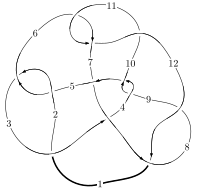
\includegraphics[width=112pt]{../../../GIT/diagram.site/Diagrams/png/2462_12n_0373.png}\\
\ \ \ A knot diagram\footnotemark}&
\allowdisplaybreaks
\textbf{Linearized knot diagam} \\
\cline{2-2}
 &
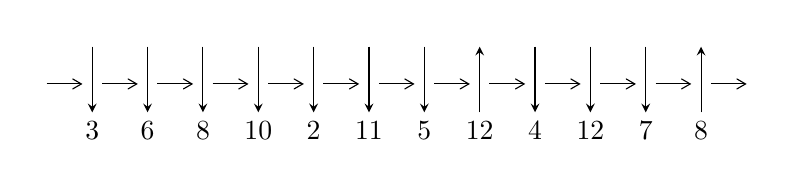
\begin{tikzpicture}[x=20pt, y=17pt]
	% nodes
	\node (C0) at (0, 0) {};
	\node (C1) at (1, 0) {};
	\node (C1U) at (1, +1) {};
	\node (C1D) at (1, -1) {3};

	\node (C2) at (2, 0) {};
	\node (C2U) at (2, +1) {};
	\node (C2D) at (2, -1) {6};

	\node (C3) at (3, 0) {};
	\node (C3U) at (3, +1) {};
	\node (C3D) at (3, -1) {8};

	\node (C4) at (4, 0) {};
	\node (C4U) at (4, +1) {};
	\node (C4D) at (4, -1) {10};

	\node (C5) at (5, 0) {};
	\node (C5U) at (5, +1) {};
	\node (C5D) at (5, -1) {2};

	\node (C6) at (6, 0) {};
	\node (C6U) at (6, +1) {};
	\node (C6D) at (6, -1) {11};

	\node (C7) at (7, 0) {};
	\node (C7U) at (7, +1) {};
	\node (C7D) at (7, -1) {5};

	\node (C8) at (8, 0) {};
	\node (C8U) at (8, +1) {};
	\node (C8D) at (8, -1) {12};

	\node (C9) at (9, 0) {};
	\node (C9U) at (9, +1) {};
	\node (C9D) at (9, -1) {4};

	\node (C10) at (10, 0) {};
	\node (C10U) at (10, +1) {};
	\node (C10D) at (10, -1) {12};

	\node (C11) at (11, 0) {};
	\node (C11U) at (11, +1) {};
	\node (C11D) at (11, -1) {7};

	\node (C12) at (12, 0) {};
	\node (C12U) at (12, +1) {};
	\node (C12D) at (12, -1) {8};
	\node (C13) at (13, 0) {};

	% arrows
	\draw[->,>={angle 60}]
	(C0) edge (C1) (C1) edge (C2) (C2) edge (C3) (C3) edge (C4) (C4) edge (C5) (C5) edge (C6) (C6) edge (C7) (C7) edge (C8) (C8) edge (C9) (C9) edge (C10) (C10) edge (C11) (C11) edge (C12) (C12) edge (C13) ;	\draw[->,>=stealth]
	(C1U) edge (C1D) (C2U) edge (C2D) (C3U) edge (C3D) (C4U) edge (C4D) (C5U) edge (C5D) (C6U) edge (C6D) (C7U) edge (C7D) (C8D) edge (C8U) (C9U) edge (C9D) (C10U) edge (C10D) (C11U) edge (C11D) (C12D) edge (C12U) ;
	\end{tikzpicture} \\
\hhline{~~} \\& 
\textbf{Solving Sequence} \\ \cline{2-2} 
 &
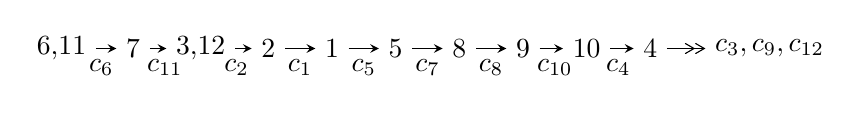
\begin{tikzpicture}[x=23pt, y=7pt]
	% node
	\node (A0) at (-1/8, 0) {6,11};
	\node (A1) at (1, 0) {7};
	\node (A2) at (33/16, 0) {3,12};
	\node (A3) at (25/8, 0) {2};
	\node (A4) at (33/8, 0) {1};
	\node (A5) at (41/8, 0) {5};
	\node (A6) at (49/8, 0) {8};
	\node (A7) at (57/8, 0) {9};
	\node (A8) at (65/8, 0) {10};
	\node (A9) at (73/8, 0) {4};
	\node (C1) at (1/2, -1) {$c_{6}$};
	\node (C2) at (3/2, -1) {$c_{11}$};
	\node (C3) at (21/8, -1) {$c_{2}$};
	\node (C4) at (29/8, -1) {$c_{1}$};
	\node (C5) at (37/8, -1) {$c_{5}$};
	\node (C6) at (45/8, -1) {$c_{7}$};
	\node (C7) at (53/8, -1) {$c_{8}$};
	\node (C8) at (61/8, -1) {$c_{10}$};
	\node (C9) at (69/8, -1) {$c_{4}$};
	\node (A10) at (11, 0) {$c_{3},c_{9},c_{12}$};

	% edge
	\draw[->,>=stealth]	
	(A0) edge (A1) (A1) edge (A2) (A2) edge (A3) (A3) edge (A4) (A4) edge (A5) (A5) edge (A6) (A6) edge (A7) (A7) edge (A8) (A8) edge (A9) ;
	\draw[->>,>={angle 60}]	
	(A9) edge (A10);
\end{tikzpicture} \\ 

\end{tabular} \\

\footnotetext{
The image of knot diagram is generated by the software ``\textbf{Draw programme}" developed by Andrew Bartholomew(\url{http://www.layer8.co.uk/maths/draw/index.htm\#Running-draw}), where we modified some parts for our purpose(\url{https://github.com/CATsTAILs/LinksPainter}).
}\phantom \\ \newline 
\centering \textbf{Ideals for irreducible components\footnotemark of $X_{\text{par}}$} 
 
\begin{align*}
I^u_{1}&=\langle 
-20 u^{23}+115 u^{22}+\cdots+8 b-400,\;113 u^{23}-773 u^{22}+\cdots+16 a+440,\;u^{24}-9 u^{23}+\cdots-144 u+32\rangle \\
I^u_{2}&=\langle 
-6 u^{15}+21 u^{14}+\cdots+b+10,\;u^{15}-6 u^{14}+\cdots+a+1,\;u^{16}-4 u^{15}+\cdots-3 u+1\rangle \\
I^u_{3}&=\langle 
2.19606\times10^{33} a^{9} u^{2}-2.28616\times10^{35} a^{8} u^{2}+\cdots+1.69568\times10^{37} a-5.01516\times10^{36},\\
\phantom{I^u_{3}}&\phantom{= \langle  }-6 a^8 u^2+14 a^7 u^2+\cdots+668 a-417,\;u^3+u^2-1\rangle \\
\\
\end{align*}
\raggedright * 3 irreducible components of $\dim_{\mathbb{C}}=0$, with total 70 representations.\\
\footnotetext{All coefficients of polynomials are rational numbers. But the coefficients are sometimes approximated in decimal forms when there is not enough margin.}
\newpage
\renewcommand{\arraystretch}{1}
\centering \section*{I. $I^u_{1}= \langle -20 u^{23}+115 u^{22}+\cdots+8 b-400,\;113 u^{23}-773 u^{22}+\cdots+16 a+440,\;u^{24}-9 u^{23}+\cdots-144 u+32 \rangle$}
\flushleft \textbf{(i) Arc colorings}\\
\begin{tabular}{m{7pt} m{180pt} m{7pt} m{180pt} }
\flushright $a_{6}=$&$\begin{pmatrix}1\\0\end{pmatrix}$ \\
\flushright $a_{11}=$&$\begin{pmatrix}0\\u\end{pmatrix}$ \\
\flushright $a_{7}=$&$\begin{pmatrix}1\\u^2\end{pmatrix}$ \\
\flushright $a_{3}=$&$\begin{pmatrix}-7.06250 u^{23}+48.3125 u^{22}+\cdots-47.5000 u-27.5000\\\frac{5}{2} u^{23}-\frac{115}{8} u^{22}+\cdots-\frac{255}{2} u+50\end{pmatrix}$ \\
\flushright $a_{12}=$&$\begin{pmatrix}- u\\- u^3+u\end{pmatrix}$ \\
\flushright $a_{2}=$&$\begin{pmatrix}-\frac{73}{16} u^{23}+\frac{543}{16} u^{22}+\cdots-175 u+\frac{45}{2}\\\frac{5}{2} u^{23}-\frac{115}{8} u^{22}+\cdots-\frac{255}{2} u+50\end{pmatrix}$ \\
\flushright $a_{1}=$&$\begin{pmatrix}-\frac{17}{8} u^{23}+\frac{141}{8} u^{22}+\cdots-\frac{783}{4} u+46\\\frac{5}{2} u^{23}-\frac{75}{4} u^{22}+\cdots+113 u-20\end{pmatrix}$ \\
\flushright $a_{5}=$&$\begin{pmatrix}-\frac{45}{32} u^{23}+\frac{511}{32} u^{22}+\cdots-324 u+\frac{183}{2}\\\frac{169}{16} u^{23}-\frac{1237}{16} u^{22}+\cdots+601 u-133\end{pmatrix}$ \\
\flushright $a_{8}=$&$\begin{pmatrix}\frac{1}{8} u^{23}-\frac{7}{8} u^{22}+\cdots+2 u+\frac{1}{2}\\-\frac{1}{4} u^{22}+\frac{7}{4} u^{21}+\cdots+\frac{27}{2} u-4\end{pmatrix}$ \\
\flushright $a_{9}=$&$\begin{pmatrix}\frac{3}{8} u^{23}-\frac{21}{8} u^{22}+\cdots+6 u+\frac{1}{2}\\\frac{1}{4} u^{23}-3 u^{22}+\cdots+\frac{147}{2} u-20\end{pmatrix}$ \\
\flushright $a_{10}=$&$\begin{pmatrix}u^3\\u^5- u^3+u\end{pmatrix}$ \\
\flushright $a_{4}=$&$\begin{pmatrix}\frac{595}{32} u^{23}-\frac{4705}{32} u^{22}+\cdots+1560 u-\frac{761}{2}\\-\frac{47}{16} u^{23}+\frac{79}{16} u^{22}+\cdots+831 u-267\end{pmatrix}$\\&\end{tabular}
\flushleft \textbf{(ii) Obstruction class $= -1$}\\~\\
\flushleft \textbf{(iii) Cusp Shapes $= -\frac{17}{4} u^{23}+\frac{127}{4} u^{22}+\cdots-152 u+18$}\\~\\
\newpage\renewcommand{\arraystretch}{1}
\flushleft \textbf{(iv) u-Polynomials at the component}\newline \\
\begin{tabular}{m{50pt}|m{274pt}}
Crossings & \hspace{64pt}u-Polynomials at each crossing \\
\hline $$\begin{aligned}c_{1}\end{aligned}$$&$\begin{aligned}
&u^{24}+7 u^{23}+\cdots+352 u+64
\end{aligned}$\\
\hline $$\begin{aligned}c_{2},c_{5}\end{aligned}$$&$\begin{aligned}
&u^{24}+7 u^{23}+\cdots-40 u-8
\end{aligned}$\\
\hline $$\begin{aligned}c_{3}\end{aligned}$$&$\begin{aligned}
&u^{24}+u^{23}+\cdots+4 u+1
\end{aligned}$\\
\hline $$\begin{aligned}c_{4},c_{7},c_{9}\end{aligned}$$&$\begin{aligned}
&u^{24}- u^{23}+\cdots+5 u^2-1
\end{aligned}$\\
\hline $$\begin{aligned}c_{6},c_{11}\end{aligned}$$&$\begin{aligned}
&u^{24}-9 u^{23}+\cdots-144 u+32
\end{aligned}$\\
\hline $$\begin{aligned}c_{8},c_{12}\end{aligned}$$&$\begin{aligned}
&u^{24}+5 u^{23}+\cdots+21 u+1
\end{aligned}$\\
\hline $$\begin{aligned}c_{10}\end{aligned}$$&$\begin{aligned}
&u^{24}+9 u^{23}+\cdots+9984 u+1024
\end{aligned}$\\
\hline
\end{tabular}\\~\\
\newpage\renewcommand{\arraystretch}{1}
\flushleft \textbf{(v) Riley Polynomials at the component}\newline \\
\begin{tabular}{m{50pt}|m{274pt}}
Crossings & \hspace{64pt}Riley Polynomials at each crossing \\
\hline $$\begin{aligned}c_{1}\end{aligned}$$&$\begin{aligned}
&y^{24}+21 y^{23}+\cdots-45568 y+4096
\end{aligned}$\\
\hline $$\begin{aligned}c_{2},c_{5}\end{aligned}$$&$\begin{aligned}
&y^{24}-7 y^{23}+\cdots-352 y+64
\end{aligned}$\\
\hline $$\begin{aligned}c_{3}\end{aligned}$$&$\begin{aligned}
&y^{24}+49 y^{23}+\cdots+36 y^2+1
\end{aligned}$\\
\hline $$\begin{aligned}c_{4},c_{7},c_{9}\end{aligned}$$&$\begin{aligned}
&y^{24}+y^{23}+\cdots-10 y+1
\end{aligned}$\\
\hline $$\begin{aligned}c_{6},c_{11}\end{aligned}$$&$\begin{aligned}
&y^{24}-9 y^{23}+\cdots-9984 y+1024
\end{aligned}$\\
\hline $$\begin{aligned}c_{8},c_{12}\end{aligned}$$&$\begin{aligned}
&y^{24}-45 y^{23}+\cdots-81 y+1
\end{aligned}$\\
\hline $$\begin{aligned}c_{10}\end{aligned}$$&$\begin{aligned}
&y^{24}+23 y^{23}+\cdots-52625408 y+1048576
\end{aligned}$\\
\hline
\end{tabular}\\~\\
\newpage\flushleft \textbf{(vi) Complex Volumes and Cusp Shapes}
$$\begin{array}{c|c|c}  
\text{Solutions to }I^u_{1}& \I (\text{vol} + \sqrt{-1}CS) & \text{Cusp shape}\\
 \hline 
\begin{aligned}
u &= \phantom{-}0.358950 + 0.915726 I \\
a &= -0.281055 + 0.691430 I \\
b &= \phantom{-}0.969760 - 0.428409 I\end{aligned}
 & \phantom{-}1.06715 + 3.63668 I & -7.18463 - 6.28452 I \\ \hline\begin{aligned}
u &= \phantom{-}0.358950 - 0.915726 I \\
a &= -0.281055 - 0.691430 I \\
b &= \phantom{-}0.969760 + 0.428409 I\end{aligned}
 & \phantom{-}1.06715 - 3.63668 I & -7.18463 + 6.28452 I \\ \hline\begin{aligned}
u &= \phantom{-}0.971229 + 0.342277 I \\
a &= -0.827201 + 0.300439 I \\
b &= -1.194730 + 0.185573 I\end{aligned}
 & -3.31191 - 1.22688 I & -3.32734 + 6.48080 I \\ \hline\begin{aligned}
u &= \phantom{-}0.971229 - 0.342277 I \\
a &= -0.827201 - 0.300439 I \\
b &= -1.194730 - 0.185573 I\end{aligned}
 & -3.31191 + 1.22688 I & -3.32734 - 6.48080 I \\ \hline\begin{aligned}
u &= \phantom{-}0.599488 + 0.713660 I \\
a &= \phantom{-}0.192159 - 1.348680 I \\
b &= \phantom{-}0.420693 + 0.742906 I\end{aligned}
 & \phantom{-}2.96075 - 0.65298 I & -2.76291 + 1.36989 I \\ \hline\begin{aligned}
u &= \phantom{-}0.599488 - 0.713660 I \\
a &= \phantom{-}0.192159 + 1.348680 I \\
b &= \phantom{-}0.420693 - 0.742906 I\end{aligned}
 & \phantom{-}2.96075 + 0.65298 I & -2.76291 - 1.36989 I \\ \hline\begin{aligned}
u &= -1.013520 + 0.559120 I \\
a &= \phantom{-}0.612654 + 0.784722 I \\
b &= -0.650003 - 0.671485 I\end{aligned}
 & -0.262441 + 0.570709 I & -9.39335 + 1.17121 I \\ \hline\begin{aligned}
u &= -1.013520 - 0.559120 I \\
a &= \phantom{-}0.612654 - 0.784722 I \\
b &= -0.650003 + 0.671485 I\end{aligned}
 & -0.262441 - 0.570709 I & -9.39335 - 1.17121 I \\ \hline\begin{aligned}
u &= \phantom{-}1.015720 + 0.612901 I \\
a &= -0.703890 + 0.704696 I \\
b &= \phantom{-}0.240215 - 0.895769 I\end{aligned}
 & \phantom{-}1.70127 - 4.44241 I & -4.62824 + 5.23976 I \\ \hline\begin{aligned}
u &= \phantom{-}1.015720 - 0.612901 I \\
a &= -0.703890 - 0.704696 I \\
b &= \phantom{-}0.240215 + 0.895769 I\end{aligned}
 & \phantom{-}1.70127 + 4.44241 I & -4.62824 - 5.23976 I\\
 \hline 
 \end{array}$$\newpage$$\begin{array}{c|c|c}  
\text{Solutions to }I^u_{1}& \I (\text{vol} + \sqrt{-1}CS) & \text{Cusp shape}\\
 \hline 
\begin{aligned}
u &= \phantom{-}0.677310 + 1.062590 I \\
a &= \phantom{-}0.57929 + 1.84135 I \\
b &= -0.833778 - 0.933127 I\end{aligned}
 & \phantom{-}10.12360 + 1.49333 I & -5.20253 - 0.24126 I \\ \hline\begin{aligned}
u &= \phantom{-}0.677310 - 1.062590 I \\
a &= \phantom{-}0.57929 - 1.84135 I \\
b &= -0.833778 + 0.933127 I\end{aligned}
 & \phantom{-}10.12360 - 1.49333 I & -5.20253 + 0.24126 I \\ \hline\begin{aligned}
u &= \phantom{-}0.668113 + 1.109120 I \\
a &= \phantom{-}0.78027 - 1.56151 I \\
b &= -1.008260 + 0.845621 I\end{aligned}
 & \phantom{-}9.55770 + 8.04939 I & -6.22396 - 5.15641 I \\ \hline\begin{aligned}
u &= \phantom{-}0.668113 - 1.109120 I \\
a &= \phantom{-}0.78027 + 1.56151 I \\
b &= -1.008260 - 0.845621 I\end{aligned}
 & \phantom{-}9.55770 - 8.04939 I & -6.22396 + 5.15641 I \\ \hline\begin{aligned}
u &= \phantom{-}1.159060 + 0.639780 I \\
a &= \phantom{-}0.61767 - 1.49231 I \\
b &= \phantom{-}1.139350 + 0.458160 I\end{aligned}
 & -1.32139 - 9.31339 I & -10.43226 + 9.48781 I \\ \hline\begin{aligned}
u &= \phantom{-}1.159060 - 0.639780 I \\
a &= \phantom{-}0.61767 + 1.49231 I \\
b &= \phantom{-}1.139350 - 0.458160 I\end{aligned}
 & -1.32139 + 9.31339 I & -10.43226 - 9.48781 I \\ \hline\begin{aligned}
u &= \phantom{-}1.122650 + 0.803919 I \\
a &= \phantom{-}1.28271 - 0.73294 I \\
b &= -0.826847 + 0.971617 I\end{aligned}
 & \phantom{-}8.67010 - 8.22857 I & -6.89988 + 3.89573 I \\ \hline\begin{aligned}
u &= \phantom{-}1.122650 - 0.803919 I \\
a &= \phantom{-}1.28271 + 0.73294 I \\
b &= -0.826847 - 0.971617 I\end{aligned}
 & \phantom{-}8.67010 + 8.22857 I & -6.89988 - 3.89573 I \\ \hline\begin{aligned}
u &= -1.39743\phantom{ +0.000000I} \\
a &= \phantom{-}0.800635\phantom{ +0.000000I} \\
b &= \phantom{-}1.04024\phantom{ +0.000000I}\end{aligned}
 & -5.27800\phantom{ +0.000000I} & -20.1480\phantom{ +0.000000I} \\ \hline\begin{aligned}
u &= \phantom{-}1.144620 + 0.817338 I \\
a &= -0.33093 + 2.27568 I \\
b &= -1.034060 - 0.861926 I\end{aligned}
 & \phantom{-}7.9963 - 14.9529 I & -7.95884 + 8.20619 I\\
 \hline 
 \end{array}$$\newpage$$\begin{array}{c|c|c}  
\text{Solutions to }I^u_{1}& \I (\text{vol} + \sqrt{-1}CS) & \text{Cusp shape}\\
 \hline 
\begin{aligned}
u &= \phantom{-}1.144620 - 0.817338 I \\
a &= -0.33093 - 2.27568 I \\
b &= -1.034060 + 0.861926 I\end{aligned}
 & \phantom{-}7.9963 + 14.9529 I & -7.95884 - 8.20619 I \\ \hline\begin{aligned}
u &= -1.32133 + 0.60253 I \\
a &= -0.32353 - 1.55196 I \\
b &= -0.992690 + 0.658211 I\end{aligned}
 & -1.26748 + 5.76484 I & -12.40197 - 1.93041 I \\ \hline\begin{aligned}
u &= -1.32133 - 0.60253 I \\
a &= -0.32353 + 1.55196 I \\
b &= -0.992690 - 0.658211 I\end{aligned}
 & -1.26748 - 5.76484 I & -12.40197 + 1.93041 I \\ \hline\begin{aligned}
u &= -0.367172\phantom{ +0.000000I} \\
a &= \phantom{-}1.00307\phantom{ +0.000000I} \\
b &= -0.499556\phantom{ +0.000000I}\end{aligned}
 & -0.751981\phantom{ +0.000000I} & -13.0200\phantom{ +0.000000I}\\
 \hline 
 \end{array}$$\newpage\newpage\renewcommand{\arraystretch}{1}
\centering \section*{II. $I^u_{2}= \langle -6 u^{15}+21 u^{14}+\cdots+b+10,\;u^{15}-6 u^{14}+\cdots+a+1,\;u^{16}-4 u^{15}+\cdots-3 u+1 \rangle$}
\flushleft \textbf{(i) Arc colorings}\\
\begin{tabular}{m{7pt} m{180pt} m{7pt} m{180pt} }
\flushright $a_{6}=$&$\begin{pmatrix}1\\0\end{pmatrix}$ \\
\flushright $a_{11}=$&$\begin{pmatrix}0\\u\end{pmatrix}$ \\
\flushright $a_{7}=$&$\begin{pmatrix}1\\u^2\end{pmatrix}$ \\
\flushright $a_{3}=$&$\begin{pmatrix}- u^{15}+6 u^{14}+\cdots+11 u-1\\6 u^{15}-21 u^{14}+\cdots+12 u-10\end{pmatrix}$ \\
\flushright $a_{12}=$&$\begin{pmatrix}- u\\- u^3+u\end{pmatrix}$ \\
\flushright $a_{2}=$&$\begin{pmatrix}5 u^{15}-15 u^{14}+\cdots+23 u-11\\6 u^{15}-21 u^{14}+\cdots+12 u-10\end{pmatrix}$ \\
\flushright $a_{1}=$&$\begin{pmatrix}-8 u^{15}+30 u^{14}+\cdots-6 u+16\\-3 u^{15}+11 u^{14}+\cdots-5 u+10\end{pmatrix}$ \\
\flushright $a_{5}=$&$\begin{pmatrix}-17 u^{15}+59 u^{14}+\cdots-40 u+35\\-10 u^{15}+35 u^{14}+\cdots-20 u+20\end{pmatrix}$ \\
\flushright $a_{8}=$&$\begin{pmatrix}2 u^{15}-7 u^{14}+\cdots+9 u-9\\u^{15}-4 u^{14}+\cdots-2 u-3\end{pmatrix}$ \\
\flushright $a_{9}=$&$\begin{pmatrix}2 u^{15}-7 u^{14}+\cdots+9 u-10\\u^{15}-4 u^{14}+\cdots-2 u-2\end{pmatrix}$ \\
\flushright $a_{10}=$&$\begin{pmatrix}u^3\\u^5- u^3+u\end{pmatrix}$ \\
\flushright $a_{4}=$&$\begin{pmatrix}-16 u^{15}+56 u^{14}+\cdots-37 u+33\\-8 u^{15}+28 u^{14}+\cdots-14 u+15\end{pmatrix}$\\&\end{tabular}
\flushleft \textbf{(ii) Obstruction class $= 1$}\\~\\
\flushleft \textbf{(iii) Cusp Shapes $= 24 u^{15}-81 u^{14}+50 u^{13}+205 u^{12}-308 u^{11}-190 u^{10}+653 u^9-51 u^8-732 u^7+325 u^6+487 u^5-327 u^4-186 u^3+183 u^2+37 u-37$}\\~\\
\newpage\renewcommand{\arraystretch}{1}
\flushleft \textbf{(iv) u-Polynomials at the component}\newline \\
\begin{tabular}{m{50pt}|m{274pt}}
Crossings & \hspace{64pt}u-Polynomials at each crossing \\
\hline $$\begin{aligned}c_{1}\end{aligned}$$&$\begin{aligned}
&u^{16}-6 u^{15}+\cdots-10 u+1
\end{aligned}$\\
\hline $$\begin{aligned}c_{2}\end{aligned}$$&$\begin{aligned}
&u^{16}-3 u^{14}+\cdots-5 u^2+1
\end{aligned}$\\
\hline $$\begin{aligned}c_{3}\end{aligned}$$&$\begin{aligned}
&u^{16}+u^{15}+\cdots- u-1
\end{aligned}$\\
\hline $$\begin{aligned}c_{4},c_{7}\end{aligned}$$&$\begin{aligned}
&u^{16}+u^{15}+\cdots+u-1
\end{aligned}$\\
\hline $$\begin{aligned}c_{5}\end{aligned}$$&$\begin{aligned}
&u^{16}-3 u^{14}+\cdots-5 u^2+1
\end{aligned}$\\
\hline $$\begin{aligned}c_{6}\end{aligned}$$&$\begin{aligned}
&u^{16}-4 u^{15}+\cdots-3 u+1
\end{aligned}$\\
\hline $$\begin{aligned}c_{8}\end{aligned}$$&$\begin{aligned}
&u^{16}- u^{15}+\cdots-8 u-1
\end{aligned}$\\
\hline $$\begin{aligned}c_{9}\end{aligned}$$&$\begin{aligned}
&u^{16}- u^{15}+\cdots- u-1
\end{aligned}$\\
\hline $$\begin{aligned}c_{10}\end{aligned}$$&$\begin{aligned}
&u^{16}-8 u^{15}+\cdots-15 u+1
\end{aligned}$\\
\hline $$\begin{aligned}c_{11}\end{aligned}$$&$\begin{aligned}
&u^{16}+4 u^{15}+\cdots+3 u+1
\end{aligned}$\\
\hline $$\begin{aligned}c_{12}\end{aligned}$$&$\begin{aligned}
&u^{16}+u^{15}+\cdots+8 u-1
\end{aligned}$\\
\hline
\end{tabular}\\~\\
\newpage\renewcommand{\arraystretch}{1}
\flushleft \textbf{(v) Riley Polynomials at the component}\newline \\
\begin{tabular}{m{50pt}|m{274pt}}
Crossings & \hspace{64pt}Riley Polynomials at each crossing \\
\hline $$\begin{aligned}c_{1}\end{aligned}$$&$\begin{aligned}
&y^{16}+14 y^{15}+\cdots-6 y+1
\end{aligned}$\\
\hline $$\begin{aligned}c_{2},c_{5}\end{aligned}$$&$\begin{aligned}
&y^{16}-6 y^{15}+\cdots-10 y+1
\end{aligned}$\\
\hline $$\begin{aligned}c_{3}\end{aligned}$$&$\begin{aligned}
&y^{16}-13 y^{15}+\cdots+25 y+1
\end{aligned}$\\
\hline $$\begin{aligned}c_{4},c_{7},c_{9}\end{aligned}$$&$\begin{aligned}
&y^{16}-13 y^{15}+\cdots-9 y+1
\end{aligned}$\\
\hline $$\begin{aligned}c_{6},c_{11}\end{aligned}$$&$\begin{aligned}
&y^{16}-8 y^{15}+\cdots-15 y+1
\end{aligned}$\\
\hline $$\begin{aligned}c_{8},c_{12}\end{aligned}$$&$\begin{aligned}
&y^{16}+9 y^{15}+\cdots-88 y+1
\end{aligned}$\\
\hline $$\begin{aligned}c_{10}\end{aligned}$$&$\begin{aligned}
&y^{16}+20 y^{15}+\cdots-31 y+1
\end{aligned}$\\
\hline
\end{tabular}\\~\\
\newpage\flushleft \textbf{(vi) Complex Volumes and Cusp Shapes}
$$\begin{array}{c|c|c}  
\text{Solutions to }I^u_{2}& \I (\text{vol} + \sqrt{-1}CS) & \text{Cusp shape}\\
 \hline 
\begin{aligned}
u &= \phantom{-}0.709766 + 0.705344 I \\
a &= -0.887882 + 0.353548 I \\
b &= -0.601245 - 0.326299 I\end{aligned}
 & -2.08950 - 3.52175 I & -8.50730 + 9.07031 I \\ \hline\begin{aligned}
u &= \phantom{-}0.709766 - 0.705344 I \\
a &= -0.887882 - 0.353548 I \\
b &= -0.601245 + 0.326299 I\end{aligned}
 & -2.08950 + 3.52175 I & -8.50730 - 9.07031 I \\ \hline\begin{aligned}
u &= -1.05256\phantom{ +0.000000I} \\
a &= \phantom{-}2.33736\phantom{ +0.000000I} \\
b &= \phantom{-}0.930995\phantom{ +0.000000I}\end{aligned}
 & -8.18293\phantom{ +0.000000I} & -21.4460\phantom{ +0.000000I} \\ \hline\begin{aligned}
u &= -0.953259 + 0.474374 I \\
a &= -0.62204 - 2.51263 I \\
b &= -0.964515 + 0.707349 I\end{aligned}
 & -3.82901 + 4.66397 I & -11.36785 - 5.44923 I \\ \hline\begin{aligned}
u &= -0.953259 - 0.474374 I \\
a &= -0.62204 + 2.51263 I \\
b &= -0.964515 - 0.707349 I\end{aligned}
 & -3.82901 - 4.66397 I & -11.36785 + 5.44923 I \\ \hline\begin{aligned}
u &= \phantom{-}1.023350 + 0.406048 I \\
a &= -0.813062 + 0.284492 I \\
b &= -1.053970 + 0.235975 I\end{aligned}
 & -3.87328 - 1.04203 I & -17.8883 + 0.9825 I \\ \hline\begin{aligned}
u &= \phantom{-}1.023350 - 0.406048 I \\
a &= -0.813062 - 0.284492 I \\
b &= -1.053970 - 0.235975 I\end{aligned}
 & -3.87328 + 1.04203 I & -17.8883 - 0.9825 I \\ \hline\begin{aligned}
u &= -0.780571 + 0.429913 I \\
a &= \phantom{-}1.97567 + 0.68038 I \\
b &= -0.759833 - 0.760705 I\end{aligned}
 & -3.18956 - 0.91432 I & -8.94555 - 0.72822 I \\ \hline\begin{aligned}
u &= -0.780571 - 0.429913 I \\
a &= \phantom{-}1.97567 - 0.68038 I \\
b &= -0.759833 + 0.760705 I\end{aligned}
 & -3.18956 + 0.91432 I & -8.94555 + 0.72822 I \\ \hline\begin{aligned}
u &= -0.656018\phantom{ +0.000000I} \\
a &= -4.43206\phantom{ +0.000000I} \\
b &= \phantom{-}0.525031\phantom{ +0.000000I}\end{aligned}
 & -6.47624\phantom{ +0.000000I} & -0.995250\phantom{ +0.000000I}\\
 \hline 
 \end{array}$$\newpage$$\begin{array}{c|c|c}  
\text{Solutions to }I^u_{2}& \I (\text{vol} + \sqrt{-1}CS) & \text{Cusp shape}\\
 \hline 
\begin{aligned}
u &= \phantom{-}1.08165 + 0.99947 I \\
a &= -0.608758 + 1.080850 I \\
b &= \phantom{-}0.755790 - 0.644213 I\end{aligned}
 & -0.62149 - 1.50137 I & -13.1344 + 5.7705 I \\ \hline\begin{aligned}
u &= \phantom{-}1.08165 - 0.99947 I \\
a &= -0.608758 - 1.080850 I \\
b &= \phantom{-}0.755790 + 0.644213 I\end{aligned}
 & -0.62149 + 1.50137 I & -13.1344 - 5.7705 I \\ \hline\begin{aligned}
u &= \phantom{-}0.498658 + 0.050338 I \\
a &= \phantom{-}1.333420 - 0.022372 I \\
b &= \phantom{-}0.939536 + 0.925652 I\end{aligned}
 & \phantom{-}5.74280 - 3.39525 I & -1.03709 + 3.22174 I \\ \hline\begin{aligned}
u &= \phantom{-}0.498658 - 0.050338 I \\
a &= \phantom{-}1.333420 + 0.022372 I \\
b &= \phantom{-}0.939536 - 0.925652 I\end{aligned}
 & \phantom{-}5.74280 + 3.39525 I & -1.03709 - 3.22174 I \\ \hline\begin{aligned}
u &= \phantom{-}1.27470 + 0.89882 I \\
a &= \phantom{-}0.17000 - 1.67912 I \\
b &= \phantom{-}0.956222 + 0.637553 I\end{aligned}
 & -1.25971 - 6.51826 I & -12.8990 + 11.7858 I \\ \hline\begin{aligned}
u &= \phantom{-}1.27470 - 0.89882 I \\
a &= \phantom{-}0.17000 + 1.67912 I \\
b &= \phantom{-}0.956222 - 0.637553 I\end{aligned}
 & -1.25971 + 6.51826 I & -12.8990 - 11.7858 I\\
 \hline 
 \end{array}$$\newpage\newpage\renewcommand{\arraystretch}{1}
\centering \section*{III. $I^u_{3}= \langle 2.20\times10^{33} a^{9} u^{2}-2.29\times10^{35} a^{8} u^{2}+\cdots+1.70\times10^{37} a-5.02\times10^{36},\;-6 a^8 u^2+14 a^7 u^2+\cdots+668 a-417,\;u^3+u^2-1 \rangle$}
\flushleft \textbf{(i) Arc colorings}\\
\begin{tabular}{m{7pt} m{180pt} m{7pt} m{180pt} }
\flushright $a_{6}=$&$\begin{pmatrix}1\\0\end{pmatrix}$ \\
\flushright $a_{11}=$&$\begin{pmatrix}0\\u\end{pmatrix}$ \\
\flushright $a_{7}=$&$\begin{pmatrix}1\\u^2\end{pmatrix}$ \\
\flushright $a_{3}=$&$\begin{pmatrix}a\\-0.0000462419 a^{9} u^{2}+0.00481392 a^{8} u^{2}+\cdots-0.357057 a+0.105603\end{pmatrix}$ \\
\flushright $a_{12}=$&$\begin{pmatrix}- u\\u^2+u-1\end{pmatrix}$ \\
\flushright $a_{2}=$&$\begin{pmatrix}-0.0000462419 a^{9} u^{2}+0.00481392 a^{8} u^{2}+\cdots+0.642943 a+0.105603\\-0.0000462419 a^{9} u^{2}+0.00481392 a^{8} u^{2}+\cdots-0.357057 a+0.105603\end{pmatrix}$ \\
\flushright $a_{1}=$&$\begin{pmatrix}0.00475440 a^{9} u^{2}+0.00480716 a^{8} u^{2}+\cdots+0.0172392 a-0.130341\\-0.00112922 a^{9} u^{2}+0.00379948 a^{8} u^{2}+\cdots-0.0267617 a+0.417054\end{pmatrix}$ \\
\flushright $a_{5}=$&$\begin{pmatrix}-0.00191453 a^{9} u^{2}+0.00196977 a^{8} u^{2}+\cdots+0.241462 a+0.176462\\-0.00155225 a^{9} u^{2}+0.00591527 a^{8} u^{2}+\cdots+0.265525 a-0.949030\end{pmatrix}$ \\
\flushright $a_{8}=$&$\begin{pmatrix}-0.000908415 a^{9} u^{2}-0.00637770 a^{8} u^{2}+\cdots-0.765719 a+0.776006\\0.00239576 a^{9} u^{2}-0.000899242 a^{8} u^{2}+\cdots-1.10079 a+0.879248\end{pmatrix}$ \\
\flushright $a_{9}=$&$\begin{pmatrix}-0.00243411 a^{9} u^{2}-0.0183142 a^{8} u^{2}+\cdots-1.55079 a+0.788681\\-0.00291032 a^{9} u^{2}+0.00645185 a^{8} u^{2}+\cdots-1.78599 a+0.677141\end{pmatrix}$ \\
\flushright $a_{10}=$&$\begin{pmatrix}- u^2+1\\u^2\end{pmatrix}$ \\
\flushright $a_{4}=$&$\begin{pmatrix}-0.00229203 a^{9} u^{2}-0.0113418 a^{8} u^{2}+\cdots+1.51032 a-0.111646\\-0.00770163 a^{9} u^{2}+0.0107723 a^{8} u^{2}+\cdots-1.51618 a-0.830861\end{pmatrix}$\\&\end{tabular}
\flushleft \textbf{(ii) Obstruction class $= -1$}\\~\\
\flushleft \textbf{(iii) Cusp Shapes $= -0.00101199 a^{9} u^{2}-0.0550471 a^{8} u^{2}+\cdots-0.470919 a-12.5272$}\\~\\
\newpage\renewcommand{\arraystretch}{1}
\flushleft \textbf{(iv) u-Polynomials at the component}\newline \\
\begin{tabular}{m{50pt}|m{274pt}}
Crossings & \hspace{64pt}u-Polynomials at each crossing \\
\hline $$\begin{aligned}c_{1}\end{aligned}$$&$\begin{aligned}
&(u^5+u^4+4 u^3+3 u^2+3 u+1)^6
\end{aligned}$\\
\hline $$\begin{aligned}c_{2},c_{5}\end{aligned}$$&$\begin{aligned}
&(u^5- u^4+u^2+u-1)^6
\end{aligned}$\\
\hline $$\begin{aligned}c_{3}\end{aligned}$$&$\begin{aligned}
&u^{30}+u^{29}+\cdots+269958 u-26963
\end{aligned}$\\
\hline $$\begin{aligned}c_{4},c_{7},c_{9}\end{aligned}$$&$\begin{aligned}
&u^{30}+u^{29}+\cdots-10 u-11
\end{aligned}$\\
\hline $$\begin{aligned}c_{6},c_{11}\end{aligned}$$&$\begin{aligned}
&(u^3+u^2-1)^{10}
\end{aligned}$\\
\hline $$\begin{aligned}c_{8},c_{12}\end{aligned}$$&$\begin{aligned}
&u^{30}+3 u^{29}+\cdots+4930 u-289
\end{aligned}$\\
\hline $$\begin{aligned}c_{10}\end{aligned}$$&$\begin{aligned}
&(u^3+u^2+2 u+1)^{10}
\end{aligned}$\\
\hline
\end{tabular}\\~\\
\newpage\renewcommand{\arraystretch}{1}
\flushleft \textbf{(v) Riley Polynomials at the component}\newline \\
\begin{tabular}{m{50pt}|m{274pt}}
Crossings & \hspace{64pt}Riley Polynomials at each crossing \\
\hline $$\begin{aligned}c_{1}\end{aligned}$$&$\begin{aligned}
&(y^5+7 y^4+16 y^3+13 y^2+3 y-1)^6
\end{aligned}$\\
\hline $$\begin{aligned}c_{2},c_{5}\end{aligned}$$&$\begin{aligned}
&(y^5- y^4+4 y^3-3 y^2+3 y-1)^6
\end{aligned}$\\
\hline $$\begin{aligned}c_{3}\end{aligned}$$&$\begin{aligned}
&y^{30}+27 y^{29}+\cdots-29765426100 y+727003369
\end{aligned}$\\
\hline $$\begin{aligned}c_{4},c_{7},c_{9}\end{aligned}$$&$\begin{aligned}
&y^{30}-9 y^{29}+\cdots+516 y+121
\end{aligned}$\\
\hline $$\begin{aligned}c_{6},c_{11}\end{aligned}$$&$\begin{aligned}
&(y^3- y^2+2 y-1)^{10}
\end{aligned}$\\
\hline $$\begin{aligned}c_{8},c_{12}\end{aligned}$$&$\begin{aligned}
&y^{30}-21 y^{29}+\cdots-50794640 y+83521
\end{aligned}$\\
\hline $$\begin{aligned}c_{10}\end{aligned}$$&$\begin{aligned}
&(y^3+3 y^2+2 y-1)^{10}
\end{aligned}$\\
\hline
\end{tabular}\\~\\
\newpage\flushleft \textbf{(vi) Complex Volumes and Cusp Shapes}
$$\begin{array}{c|c|c}  
\text{Solutions to }I^u_{3}& \I (\text{vol} + \sqrt{-1}CS) & \text{Cusp shape}\\
 \hline 
\begin{aligned}
u &= -0.877439 + 0.744862 I \\
a &= \phantom{-}0.283563 + 0.915777 I \\
b &= -0.758138 - 0.584034 I\end{aligned}
 & -0.090868 + 0.614153 I & -7.60456 + 1.24344 I \\ \hline\begin{aligned}
u &= -0.877439 + 0.744862 I \\
a &= \phantom{-}1.019500 + 0.839116 I \\
b &= -0.758138 - 0.584034 I\end{aligned}
 & -0.090868 + 0.614153 I & -7.60456 + 1.24344 I \\ \hline\begin{aligned}
u &= -0.877439 + 0.744862 I \\
a &= \phantom{-}0.038650 - 1.390540 I \\
b &= -0.758138 + 0.584034 I\end{aligned}
 & -0.09087 + 5.04209 I & -7.60456 - 7.20234 I \\ \hline\begin{aligned}
u &= -0.877439 + 0.744862 I \\
a &= \phantom{-}0.073356 - 0.330206 I \\
b &= \phantom{-}0.645200\phantom{ +0.000000I}\end{aligned}
 & -2.79286 + 2.82812 I & -16.0991 - 2.9794 I \\ \hline\begin{aligned}
u &= -0.877439 + 0.744862 I \\
a &= \phantom{-}1.24901 + 1.29138 I \\
b &= \phantom{-}0.645200\phantom{ +0.000000I}\end{aligned}
 & -2.79286 + 2.82812 I & -16.0991 - 2.9794 I \\ \hline\begin{aligned}
u &= -0.877439 + 0.744862 I \\
a &= -1.00422 - 1.60730 I \\
b &= \phantom{-}0.935538 + 0.903908 I\end{aligned}
 & \phantom{-}9.04762 - 0.50362 I & -6.57151 - 0.61717 I \\ \hline\begin{aligned}
u &= -0.877439 + 0.744862 I \\
a &= -1.81399 - 0.55743 I \\
b &= \phantom{-}0.935538 + 0.903908 I\end{aligned}
 & \phantom{-}9.04762 - 0.50362 I & -6.57151 - 0.61717 I \\ \hline\begin{aligned}
u &= -0.877439 + 0.744862 I \\
a &= -0.58303 + 2.03306 I \\
b &= \phantom{-}0.935538 - 0.903908 I\end{aligned}
 & \phantom{-}9.04762 + 6.15987 I & -6.57151 - 5.34173 I \\ \hline\begin{aligned}
u &= -0.877439 + 0.744862 I \\
a &= -0.47568 - 2.62318 I \\
b &= -0.758138 + 0.584034 I\end{aligned}
 & -0.09087 + 5.04209 I & -7.60456 - 7.20234 I \\ \hline\begin{aligned}
u &= -0.877439 + 0.744862 I \\
a &= \phantom{-}0.45796 + 2.91906 I \\
b &= \phantom{-}0.935538 - 0.903908 I\end{aligned}
 & \phantom{-}9.04762 + 6.15987 I & -6.57151 - 5.34173 I\\
 \hline 
 \end{array}$$\newpage$$\begin{array}{c|c|c}  
\text{Solutions to }I^u_{3}& \I (\text{vol} + \sqrt{-1}CS) & \text{Cusp shape}\\
 \hline 
\begin{aligned}
u &= -0.877439 - 0.744862 I \\
a &= \phantom{-}0.283563 - 0.915777 I \\
b &= -0.758138 + 0.584034 I\end{aligned}
 & -0.090868 - 0.614153 I & -7.60456 - 1.24344 I \\ \hline\begin{aligned}
u &= -0.877439 - 0.744862 I \\
a &= \phantom{-}1.019500 - 0.839116 I \\
b &= -0.758138 + 0.584034 I\end{aligned}
 & -0.090868 - 0.614153 I & -7.60456 - 1.24344 I \\ \hline\begin{aligned}
u &= -0.877439 - 0.744862 I \\
a &= \phantom{-}0.038650 + 1.390540 I \\
b &= -0.758138 - 0.584034 I\end{aligned}
 & -0.09087 - 5.04209 I & -7.60456 + 7.20234 I \\ \hline\begin{aligned}
u &= -0.877439 - 0.744862 I \\
a &= \phantom{-}0.073356 + 0.330206 I \\
b &= \phantom{-}0.645200\phantom{ +0.000000I}\end{aligned}
 & -2.79286 - 2.82812 I & -16.0991 + 2.9794 I \\ \hline\begin{aligned}
u &= -0.877439 - 0.744862 I \\
a &= \phantom{-}1.24901 - 1.29138 I \\
b &= \phantom{-}0.645200\phantom{ +0.000000I}\end{aligned}
 & -2.79286 - 2.82812 I & -16.0991 + 2.9794 I \\ \hline\begin{aligned}
u &= -0.877439 - 0.744862 I \\
a &= -1.00422 + 1.60730 I \\
b &= \phantom{-}0.935538 - 0.903908 I\end{aligned}
 & \phantom{-}9.04762 + 0.50362 I & -6.57151 + 0.61717 I \\ \hline\begin{aligned}
u &= -0.877439 - 0.744862 I \\
a &= -1.81399 + 0.55743 I \\
b &= \phantom{-}0.935538 - 0.903908 I\end{aligned}
 & \phantom{-}9.04762 + 0.50362 I & -6.57151 + 0.61717 I \\ \hline\begin{aligned}
u &= -0.877439 - 0.744862 I \\
a &= -0.58303 - 2.03306 I \\
b &= \phantom{-}0.935538 + 0.903908 I\end{aligned}
 & \phantom{-}9.04762 - 6.15987 I & -6.57151 + 5.34173 I \\ \hline\begin{aligned}
u &= -0.877439 - 0.744862 I \\
a &= -0.47568 + 2.62318 I \\
b &= -0.758138 - 0.584034 I\end{aligned}
 & -0.09087 - 5.04209 I & -7.60456 + 7.20234 I \\ \hline\begin{aligned}
u &= -0.877439 - 0.744862 I \\
a &= \phantom{-}0.45796 - 2.91906 I \\
b &= \phantom{-}0.935538 + 0.903908 I\end{aligned}
 & \phantom{-}9.04762 - 6.15987 I & -6.57151 + 5.34173 I\\
 \hline 
 \end{array}$$\newpage$$\begin{array}{c|c|c}  
\text{Solutions to }I^u_{3}& \I (\text{vol} + \sqrt{-1}CS) & \text{Cusp shape}\\
 \hline 
\begin{aligned}
u &= \phantom{-}0.754878\phantom{ +0.000000I} \\
a &= -0.152878 + 1.046890 I \\
b &= \phantom{-}0.935538 - 0.903908 I\end{aligned}
 & \phantom{-}4.91003 + 3.33174 I & -13.10077 - 2.36228 I \\ \hline\begin{aligned}
u &= \phantom{-}0.754878\phantom{ +0.000000I} \\
a &= -0.152878 - 1.046890 I \\
b &= \phantom{-}0.935538 + 0.903908 I\end{aligned}
 & \phantom{-}4.91003 - 3.33174 I & -13.10077 + 2.36228 I \\ \hline\begin{aligned}
u &= \phantom{-}0.754878\phantom{ +0.000000I} \\
a &= \phantom{-}0.997843 + 0.652805 I \\
b &= -0.758138 + 0.584034 I\end{aligned}
 & -4.22845 + 2.21397 I & -14.1338 - 4.2229 I \\ \hline\begin{aligned}
u &= \phantom{-}0.754878\phantom{ +0.000000I} \\
a &= \phantom{-}0.997843 - 0.652805 I \\
b &= -0.758138 - 0.584034 I\end{aligned}
 & -4.22845 - 2.21397 I & -14.1338 + 4.2229 I \\ \hline\begin{aligned}
u &= \phantom{-}0.754878\phantom{ +0.000000I} \\
a &= \phantom{-}1.73543 + 0.43939 I \\
b &= \phantom{-}0.935538 + 0.903908 I\end{aligned}
 & \phantom{-}4.91003 - 3.33174 I & -13.10077 + 2.36228 I \\ \hline\begin{aligned}
u &= \phantom{-}0.754878\phantom{ +0.000000I} \\
a &= \phantom{-}1.73543 - 0.43939 I \\
b &= \phantom{-}0.935538 - 0.903908 I\end{aligned}
 & \phantom{-}4.91003 + 3.33174 I & -13.10077 - 2.36228 I \\ \hline\begin{aligned}
u &= \phantom{-}0.754878\phantom{ +0.000000I} \\
a &= -2.59655\phantom{ +0.000000I} \\
b &= \phantom{-}0.645200\phantom{ +0.000000I}\end{aligned}
 & -6.93044\phantom{ +0.000000I} & -22.6280\phantom{ +0.000000I} \\ \hline\begin{aligned}
u &= \phantom{-}0.754878\phantom{ +0.000000I} \\
a &= -3.03987 + 1.63046 I \\
b &= -0.758138 - 0.584034 I\end{aligned}
 & -4.22845 - 2.21397 I & -14.1338 + 4.2229 I \\ \hline\begin{aligned}
u &= \phantom{-}0.754878\phantom{ +0.000000I} \\
a &= -3.03987 - 1.63046 I \\
b &= -0.758138 + 0.584034 I\end{aligned}
 & -4.22845 + 2.21397 I & -14.1338 - 4.2229 I \\ \hline\begin{aligned}
u &= \phantom{-}0.754878\phantom{ +0.000000I} \\
a &= \phantom{-}6.02526\phantom{ +0.000000I} \\
b &= \phantom{-}0.645200\phantom{ +0.000000I}\end{aligned}
 & -6.93044\phantom{ +0.000000I} & -22.6280\phantom{ +0.000000I}\\
 \hline 
 \end{array}$$\newpage
\newpage\renewcommand{\arraystretch}{1}
\centering \section*{ IV. u-Polynomials}
\begin{tabular}{m{50pt}|m{274pt}}
Crossings & \hspace{64pt}u-Polynomials at each crossing \\
\hline $$\begin{aligned}c_{1}\end{aligned}$$&$\begin{aligned}
&((u^5+u^4+4 u^3+3 u^2+3 u+1)^6)(u^{16}-6 u^{15}+\cdots-10 u+1)\\
&\cdot(u^{24}+7 u^{23}+\cdots+352 u+64)
\end{aligned}$\\
\hline $$\begin{aligned}c_{2}\end{aligned}$$&$\begin{aligned}
&((u^5- u^4+u^2+u-1)^6)(u^{16}-3 u^{14}+\cdots-5 u^2+1)\\
&\cdot(u^{24}+7 u^{23}+\cdots-40 u-8)
\end{aligned}$\\
\hline $$\begin{aligned}c_{3}\end{aligned}$$&$\begin{aligned}
&(u^{16}+u^{15}+\cdots- u-1)(u^{24}+u^{23}+\cdots+4 u+1)\\
&\cdot(u^{30}+u^{29}+\cdots+269958 u-26963)
\end{aligned}$\\
\hline $$\begin{aligned}c_{4},c_{7}\end{aligned}$$&$\begin{aligned}
&(u^{16}+u^{15}+\cdots+u-1)(u^{24}- u^{23}+\cdots+5 u^2-1)\\
&\cdot(u^{30}+u^{29}+\cdots-10 u-11)
\end{aligned}$\\
\hline $$\begin{aligned}c_{5}\end{aligned}$$&$\begin{aligned}
&((u^5- u^4+u^2+u-1)^6)(u^{16}-3 u^{14}+\cdots-5 u^2+1)\\
&\cdot(u^{24}+7 u^{23}+\cdots-40 u-8)
\end{aligned}$\\
\hline $$\begin{aligned}c_{6}\end{aligned}$$&$\begin{aligned}
&((u^3+u^2-1)^{10})(u^{16}-4 u^{15}+\cdots-3 u+1)(u^{24}-9 u^{23}+\cdots-144 u+32)
\end{aligned}$\\
\hline $$\begin{aligned}c_{8}\end{aligned}$$&$\begin{aligned}
&(u^{16}- u^{15}+\cdots-8 u-1)(u^{24}+5 u^{23}+\cdots+21 u+1)\\
&\cdot(u^{30}+3 u^{29}+\cdots+4930 u-289)
\end{aligned}$\\
\hline $$\begin{aligned}c_{9}\end{aligned}$$&$\begin{aligned}
&(u^{16}- u^{15}+\cdots- u-1)(u^{24}- u^{23}+\cdots+5 u^2-1)\\
&\cdot(u^{30}+u^{29}+\cdots-10 u-11)
\end{aligned}$\\
\hline $$\begin{aligned}c_{10}\end{aligned}$$&$\begin{aligned}
&((u^3+u^2+2 u+1)^{10})(u^{16}-8 u^{15}+\cdots-15 u+1)\\
&\cdot(u^{24}+9 u^{23}+\cdots+9984 u+1024)
\end{aligned}$\\
\hline $$\begin{aligned}c_{11}\end{aligned}$$&$\begin{aligned}
&((u^3+u^2-1)^{10})(u^{16}+4 u^{15}+\cdots+3 u+1)(u^{24}-9 u^{23}+\cdots-144 u+32)
\end{aligned}$\\
\hline $$\begin{aligned}c_{12}\end{aligned}$$&$\begin{aligned}
&(u^{16}+u^{15}+\cdots+8 u-1)(u^{24}+5 u^{23}+\cdots+21 u+1)\\
&\cdot(u^{30}+3 u^{29}+\cdots+4930 u-289)
\end{aligned}$\\
\hline
\end{tabular}\newpage\renewcommand{\arraystretch}{1}
\centering \section*{ V. Riley Polynomials}
\begin{tabular}{m{50pt}|m{274pt}}
Crossings & \hspace{64pt}Riley Polynomials at each crossing \\
\hline $$\begin{aligned}c_{1}\end{aligned}$$&$\begin{aligned}
&((y^5+7 y^4+16 y^3+13 y^2+3 y-1)^{6})(y^{16}+14 y^{15}+\cdots-6 y+1)\\
&\cdot(y^{24}+21 y^{23}+\cdots-45568 y+4096)
\end{aligned}$\\
\hline $$\begin{aligned}c_{2},c_{5}\end{aligned}$$&$\begin{aligned}
&((y^5- y^4+4 y^3-3 y^2+3 y-1)^6)(y^{16}-6 y^{15}+\cdots-10 y+1)\\
&\cdot(y^{24}-7 y^{23}+\cdots-352 y+64)
\end{aligned}$\\
\hline $$\begin{aligned}c_{3}\end{aligned}$$&$\begin{aligned}
&(y^{16}-13 y^{15}+\cdots+25 y+1)(y^{24}+49 y^{23}+\cdots+36 y^2+1)\\
&\cdot(y^{30}+27 y^{29}+\cdots-29765426100 y+727003369)
\end{aligned}$\\
\hline $$\begin{aligned}c_{4},c_{7},c_{9}\end{aligned}$$&$\begin{aligned}
&(y^{16}-13 y^{15}+\cdots-9 y+1)(y^{24}+y^{23}+\cdots-10 y+1)\\
&\cdot(y^{30}-9 y^{29}+\cdots+516 y+121)
\end{aligned}$\\
\hline $$\begin{aligned}c_{6},c_{11}\end{aligned}$$&$\begin{aligned}
&((y^3- y^2+2 y-1)^{10})(y^{16}-8 y^{15}+\cdots-15 y+1)\\
&\cdot(y^{24}-9 y^{23}+\cdots-9984 y+1024)
\end{aligned}$\\
\hline $$\begin{aligned}c_{8},c_{12}\end{aligned}$$&$\begin{aligned}
&(y^{16}+9 y^{15}+\cdots-88 y+1)(y^{24}-45 y^{23}+\cdots-81 y+1)\\
&\cdot(y^{30}-21 y^{29}+\cdots-50794640 y+83521)
\end{aligned}$\\
\hline $$\begin{aligned}c_{10}\end{aligned}$$&$\begin{aligned}
&((y^3+3 y^2+2 y-1)^{10})(y^{16}+20 y^{15}+\cdots-31 y+1)\\
&\cdot(y^{24}+23 y^{23}+\cdots-52625408 y+1048576)
\end{aligned}$\\
\hline
\end{tabular}
\vskip 2pc
\end{document}